\documentclass[12pt,a4paper]{article}

% ----- CÁC GÓI HỖ TRỢ TIẾNG VIỆT VÀ ĐỊNH DẠNG -----
\usepackage[utf8]{inputenc} % Bảng mã UTF-8
\usepackage[T5]{fontenc}    % Font tiếng Việt
\usepackage[vietnamese]{babel} % Ngôn ngữ tiếng Việt
\usepackage{mathptmx} % Font Times New Roman tương đương
\usepackage{indentfirst} % Thụt đầu dòng đoạn đầu tiên

\usepackage[margin=2.5cm]{geometry} % Căn lề giấy
\usepackage{graphicx}       % Hỗ trợ chèn ảnh
\usepackage{hyperref}       % Tạo link click được cho Mục lục
\usepackage{titlesec}       % Tùy chỉnh tiêu đề
\usepackage{listings}       % Hỗ trợ chèn code
\usepackage{xcolor}         % Hỗ trợ màu sắc cho code và text
\usepackage{array}
\usepackage{enumitem} 
\usepackage{longtable}
\setlist{nosep} % Loại bỏ khoảng trắng thừa giữa các dòng
\setlist[itemize]{leftmargin=*} % Căn lề thông minh cho gạch đầu dòng
\setlist[enumerate]{leftmargin=*} % Căn lề thông minh cho số thứ tự

% --- Cấu hình giãn dòng ---
\usepackage{setspace}
\setstretch{1.3} % Thiết lập giãn dòng 1.3 cho toàn bộ tài liệu

% Cài đặt màu và định dạng cho phần chèn code
\definecolor{codegreen}{rgb}{0,0.6,0}
\definecolor{codegray}{rgb}{0.5,0.5,0.5}
\definecolor{codepurple}{rgb}{0.58,0,0.82}
\definecolor{backcolour}{rgb}{0.95,0.95,0.92}

\lstdefinestyle{mystyle}{   
    backgroundcolor=\color{backcolour},   
    commentstyle=\color{codegreen},
    keywordstyle=\color{magenta},
    numberstyle=\tiny\color{codegray},
    stringstyle=\color{codepurple},
    basicstyle=\ttfamily\footnotesize,
    breakatwhitespace=false,         
    breaklines=true,                 
    captionpos=b,                    
    keepspaces=true,                 
    numbers=left,                    
    numbersep=5pt,                  
    showspaces=false,                
    showstringspaces=false,
    showtabs=false,                  
    tabsize=2
}
\lstset{style=mystyle}

% Định dạng link ẩn khung viền đỏ
\hypersetup{
    colorlinks=true,
    linkcolor=black,
    filecolor=blue,      
    urlcolor=blue,
    citecolor=black,
}

\begin{document}


% ==========================================
% TRANG BÌA
% ==========================================
\begin{titlepage}
    \begin{center}
        \textbf{\large ĐẠI HỌC QUỐC GIA THÀNH PHỐ HỒ CHÍ MINH}\\
        \textbf{\large TRƯỜNG ĐẠI HỌC KHOA HỌC TỰ NHIÊN}\\
        \textbf{\large KHOA CÔNG NGHỆ THÔNG TIN}
        
        \vspace{3cm}
        
        
\includegraphics[width=0.4\textwidth]{assets/logo-hcmus.png}
        
        \vspace{2cm}
        
        {\LARGE \textbf{BÁO CÁO ĐỒ ÁN MÔN HỌC}}\\
        \vspace{0.5cm}
        {\Huge \textbf{Toán ứng dụng và thống kê}}\\
        
        \vspace{2cm}
        
        \begin{table}[h]
            \centering
            \begin{tabular}{ll}
                \textbf{Giáo viên hướng dẫn:} & ThS. Lê Nhựt Nam \\
                                            & ThS. Võ Nam Thục Đoan \\
                                            & \\
                \textbf{Nhóm thực hiện:} & Nhóm 3 - Lớp 24CTT2 \\
                \textbf{Thành viên:} & 24120018 – Đào Thị Quỳnh Anh \\
                                     & 24120347 - Phan Lê Đăng Khoa \\ 
                                     & 24120348 – Hà Đăng Khôi \\
                                     & 24120352 – Lương Trung Kiên \\
                                     & 24120418 – Nguyễn Minh Quân \\
            \end{tabular}
        \end{table}
        
        \vfill
        
        \textbf{Hồ Chí Minh, 2026}
    \end{center}
\end{titlepage}

% ==========================================
% MỤC LỤC
% ==========================================
\tableofcontents
\newpage

\listoffigures % Danh mục hình ảnh
\newpage

% ==========================================
% NỘI DUNG CHÍNH 
% ==========================================

% Phân công công việc
% ==========================================
% BẢNG PHÂN CÔNG CÔNG VIỆC
% ==========================================
\section*{BẢNG PHÂN CÔNG CÔNG VIỆC VÀ MỨC ĐỘ ĐÓNG GÓP}
\addcontentsline{toc}{section}{Bảng phân công công việc}

\renewcommand{\arraystretch}{1.5}
% Thay tabular bằng longtable
\begin{longtable}{|p{0.05\textwidth}|p{0.18\textwidth}|>{\linespread{1.3}\selectfont\arraybackslash}p{0.6\textwidth}|p{0.08\textwidth}|}
    
    % --- 1. TIÊU ĐỀ Ở TRANG ĐẦU TIÊN ---
    \hline
    \centering \textbf{STT} & \textbf{Họ tên / MSSV} & \textbf{Nhiệm vụ đảm nhiệm chi tiết} & \textbf{Đóng góp} \\ \hline
    \endfirsthead
    
    % --- 2. TIÊU ĐỀ LẶP LẠI Ở CÁC TRANG SAU ---
    \hline
    \centering \textbf{STT} & \textbf{Họ tên / MSSV} & \textbf{Nhiệm vụ đảm nhiệm chi tiết} & \textbf{Đóng góp} \\ \hline
    \endhead
    
    % --- 3. CHÂN BẢNG Ở CÁC TRANG BỊ NGẮT ---
    \hline
    \endfoot
    
    % --- 4. CHÂN BẢNG Ở TRANG CUỐI CÙNG ---
    \hline
    \endlastfoot

    % ================= NỘI DUNG BẢNG =================
    
    % Thành viên 1
    \centering 1 & 
    24120018 \newline \textbf{Đào Thị Quỳnh Anh} & 
    \vspace{-0.4cm}
    \begin{itemize}[itemsep=0.15cm, topsep=0cm, partopsep=0cm]
        \item Biên soạn \texttt{part1\_demo.ipynb} minh họa trực quan kết quả Phần 1.
        \item Xây dựng \texttt{data\_gen.py}: Viết script sinh ma trận ngẫu nhiên SPD (well-conditioned) và ma trận Hilbert $H_n$ (ill-conditioned).
        \item Phân tích tính ổn định: Tính số điều kiện $\kappa_2(A)$, thu thập sai số tương đối và lý luận giải thích hiện tượng theo Định lý 3.1.
    \end{itemize} \vspace{-0.2cm} & 
    \centering 100\% \tabularnewline \hline
    
    % Thành viên 2
    \centering 2 & 
    24120347 \newline \textbf{Phan Lê Đăng Khoa} & 
    \vspace{-0.4cm}
    \begin{itemize}[itemsep=0.15cm, topsep=0cm, partopsep=0cm]
        \item Cài đặt thuật toán phân rã SVD (Phần 2).
        \item Xây dựng \texttt{solvers.py}: Tích hợp phương pháp Gauss, SVD và cài đặt thuật toán lặp Gauss-Seidel (kèm hàm kiểm tra ma trận chéo trội).
        \item Xây dựng \texttt{benchmark.py}: Lên kịch bản đo thời gian thực thi (trung bình 5 vòng lặp), tính sai số tương đối và xuất dữ liệu ra định dạng JSON chuẩn.
    \end{itemize} \vspace{-0.2cm} & 
    \centering 100\% \tabularnewline \hline
    
    % Thành viên 3
    \centering 3 & 
    24120348 \newline \textbf{Hà Đăng Khôi} & 
    \vspace{-0.4cm}
    \begin{itemize}[itemsep=0.15cm, topsep=0cm, partopsep=0cm]
        \item Trực quan hóa Toán học (Phần 2): Viết kịch bản và lập trình tạo Video demo hoạt ảnh quá trình phân rã ma trận bằng thư viện Manim.
        \item Phối hợp viết báo cáo tổng kết, biên tập tài liệu và quay dựng thành phẩm nộp bài cuối cùng.
    \end{itemize} \vspace{-0.2cm} & 
    \centering 100\% \tabularnewline \hline

    % Thành viên 4
    \centering 4 & 
    24120352 \newline \textbf{Lương Trung Kiên} & 
    \vspace{-0.4cm}
    \begin{itemize}[itemsep=0.15cm, topsep=0cm, partopsep=0cm]
        \item Phối hợp cài đặt thuật toán Phép khử Gauss và ứng dụng (Phần 1).
        \item Xây dựng \texttt{analysis.ipynb} (Phần 3): Đọc file dữ liệu JSON, vẽ đồ thị log-log so sánh thời gian thực tế với đường lý thuyết $O(n^3)$.
        \item Trình bày Markdown lý thuyết Toán học (số điều kiện, Gauss-Seidel) và viết kết luận đánh giá tương quan giữa tính ổn định và chi phí tính toán.
    \end{itemize} \vspace{-0.2cm} & 
    \centering 100\% \tabularnewline \hline
    
    % Thành viên 5
    \centering 5 & 
    24120418 \newline \textbf{Nguyễn Minh Quân} & 
    \vspace{-0.4cm}
    \begin{itemize}[itemsep=0.15cm, topsep=0cm, partopsep=0cm]
        \item Phối hợp cài đặt thuật toán Phép khử Gauss và ứng dụng (Phần 1).
        \item Biên soạn Báo cáo bằng \LaTeX (\texttt{report.tex}): Dựng khung tài liệu, xử lý các môi trường công thức Toán học phức tạp cho Phần 1 và Phần 2.
        \item Trích xuất dữ liệu, chèn biểu đồ từ Notebook vào báo cáo, viết phần Mở đầu, Kết luận và rà soát toàn bộ source code trước khi nộp.
    \end{itemize} \vspace{-0.2cm} & 
    \centering 100\% \tabularnewline \hline
    
\end{longtable}
\newpage

\section{Phần 1: Phép khử Gauss và Các Ứng Dụng}
Trong phần này, nhóm tiến hành cài đặt phương pháp khử Gauss có chọn phần tử chốt (Partial Pivoting) từ đầu bằng Python...

\subsection{Cơ sở lý thuyết}
Nội dung cơ sở lý thuyết về phép khử Gauss, định nghĩa ma trận tăng cường, các phép biến đổi dòng sơ cấp...

\subsection{Cài đặt thuật toán}
Trình bày về cấu trúc hàm \texttt{gaussian\_eliminate(A, b)}...

\begin{lstlisting}[language=Python, caption=code mẫu]
import numpy as np

def process_data(data_path):
    print("Code minh hoa chen tai phu luc...")
    return True
\end{lstlisting}

\subsection{Kiểm thử và đối chiếu kết quả}

\subsubsection{Phương pháp đo lường sai số}
Để đánh giá tính đúng đắn và độ ổn định của thuật toán Khử Gauss tự cài đặt (Custom Solver), nhóm không chỉ so sánh trực tiếp vector nghiệm $x$ thu được với kết quả từ thư viện \texttt{numpy.linalg.solve}, mà còn sử dụng \textbf{Chuẩn L2 của vector phần dư (Residual Norm)} làm thước đo chính:
\begin{equation}
    e = ||r||_2 = ||b - Ax||_2 = \sqrt{\sum_{i=1}^{n} (b_i - (Ax)_i)^2}
\end{equation}
Việc đo lường sai số phần dư giúp phản ánh chính xác chất lượng của nghiệm đối với cấu trúc ma trận $A$ ban đầu, đặc biệt hữu ích khi đánh giá các hệ phương trình nhạy cảm với nhiễu.

\subsubsection{Kịch bản kiểm thử và kết quả thực nghiệm}
Nhóm đã xây dựng một bộ Test Suite gồm 7 kịch bản, bao phủ từ các trường hợp cơ bản đến các "điểm chết" của chuẩn biểu diễn dấu phẩy động IEEE 754 (Double Precision).

\vspace{0.3cm}
\begin{center}
    \renewcommand{\arraystretch}{1.4}
    \begin{tabular}{|c|p{0.3\textwidth}|p{0.3\textwidth}|c|}
        \hline
        \textbf{STT} & \textbf{Kịch bản kiểm thử (Test Case)} & \textbf{Ý nghĩa kiểm tra} & \textbf{Sai số L2 ($e$)} \\ \hline
        1 & Hệ cơ bản (Nghiệm nguyên) & Tính đúng đắn của thuật toán & $0.00e+00$ \\ \hline
        2 & Nhiễu làm tròn (Round-off) & Phép chia cho số vô hạn tuần hoàn & $5.55e-17$ \\ \hline
        3 & Cần Partial Pivoting & Khử phần tử chốt (pivot) tiệm cận 0 & $0.00e+00$ \\ \hline
        4 & Chênh lệch hệ số khổng lồ & Hiện tượng nuốt số (Swamping) & $0.00e+00$ \\ \hline
        5 & Hệ điều kiện kém (Near-singular) & Khuếch đại sai số do hai dòng gần song song & $2.22e-16$ \\ \hline
        6 & Ma trận Hilbert 3x3 & Ma trận có số điều kiện lớn & $1.11e-16$ \\ \hline
        7 & Ma trận suy biến & Khả năng bắt lỗi hệ vô số nghiệm/vô nghiệm & Không có nghiệm \\ \hline
    \end{tabular}
\end{center}
\vspace{0.3cm}

\subsubsection{Phân tích các vấn đề và hiện tượng sai số}

Dựa trên kết quả thực nghiệm, nhóm rút ra các phân tích sâu sắc về bản chất của tính toán số học trên máy tính:

\textbf{a) Vấn đề 1: Nhiễu làm tròn số} \\
Ở Kịch bản 1, sai số trả về là $0.00$. Tuy nhiên, ở Kịch bản 2, dù thuật toán chạy đúng, sai số phần dư vẫn nhích lên mức $5.55 \times 10^{-17}$. Nguyên nhân là do các phân số như $1/3$ hoặc số thập phân như $0.1$ khi chuyển sang hệ nhị phân sẽ trở thành chuỗi vô hạn tuần hoàn. Máy tính bị giới hạn bởi bộ nhớ 64-bit nên buộc phải cắt bớt phần đuôi, sinh ra \textbf{Machine Epsilon} (độ phân giải máy tính $\approx 2.22 \times 10^{-16}$). Mức sai số này là giới hạn vật lý của phần cứng, không phải lỗi của thuật toán.

\textbf{b) Vấn đề 2: Hiện tượng Swamping và vai trò của Partial Pivoting} \\
Ở Kịch bản 4, hệ phương trình chứa phép cộng giữa một số khổng lồ ($10^{15}$) và một số rất nhỏ ($1.0$). Nếu thuật toán giữ nguyên dòng đầu tiên làm phần tử chốt, số $1.0$ sẽ mất hoàn toàn trong cấu trúc bộ nhớ \textit{Mantissa}, dẫn đến sự triệt tiêu. Nhờ áp dụng chiến lược \textbf{Partial Pivoting} (Hoán đổi dòng), thuật toán đã đưa hệ số an toàn nhất lên làm chốt, giúp triệt tiêu hoàn toàn sai số và giữ được $e = 0.00$.

\textbf{c) Vấn đề 3: Sự khuếch đại sai số ở Hệ điều kiện kém (Ill-conditioned System)} \\
Đây là hiện tượng Toán học đáng chú ý nhất ở Kịch bản 5 và 6. Ở Kịch bản 5, ma trận chứa hai hàng gần như song song (hệ số lệch nhau ở chữ số thập phân thứ 15). Dù nhiễu làm tròn ở cấp số $10^{-16}$, nhưng do \textbf{Số điều kiện (Condition Number)} của ma trận quá khổng lồ, nó đã đóng vai trò như một bộ khuếch đại tín hiệu xấu.
Hậu quả là nghiệm tính ra bị "trôi dạt" (Drift) sai lệch hẳn so với nghiệm lý thuyết, dù khi thế ngược vào phương trình thì sai số phần dư $e$ vẫn rất nhỏ ($2.22 \times 10^{-16}$). Điều này khẳng định: Với hệ điều kiện kém, sai số dư nhỏ không đồng nghĩa với vector nghiệm có độ chính xác cao.

\vspace{0.3cm}
\textbf{Kết luận Phần 1:} Đồ thị log-log đo lường hiệu năng (được trình bày trong Jupyter Notebook) cho thấy đường sai số của thuật toán tự cài đặt hoàn toàn trùng khớp và bám sát với thư viện \texttt{LAPACK} siêu tối ưu của NumPy. Thuật toán đã xử lý thành công mọi góc khuất của hệ thống số dấu phẩy động.

\begin{figure}[h]
    \centering
    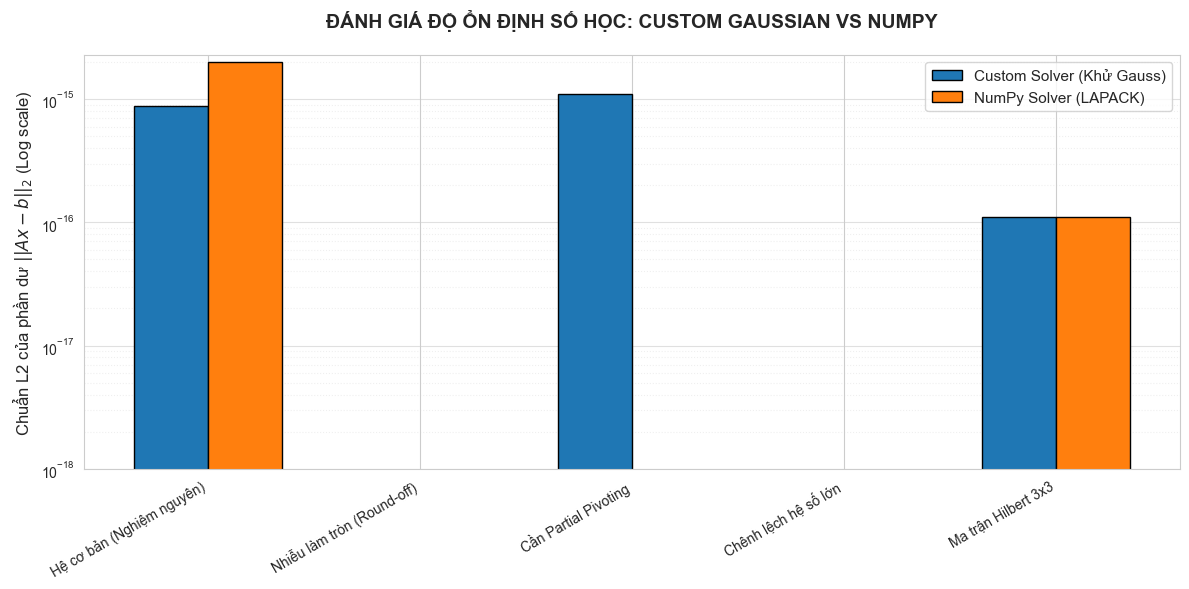
\includegraphics[width=\textwidth]{assets/part1-error.png}
    \caption{Đánh giá độ ổn định số học: Custom Gaussian vs NumPy}
    \label{fig:part1_demo}
\end{figure}
\newpage

\section{Phần 2: Phân Rã Ma Trận và Trực Quan Hóa với Manim}
Nội dung chi tiết của phần 2...

\subsection{Cơ sở lý thuyết phương pháp phân rã}
Mô tả phương pháp (LU, QR, SVD, hoặc Cholesky) mà nhóm đã chọn.

\subsection{Chéo hóa ma trận}
Trình bày việc cài đặt tìm giá trị riêng, vector riêng...

\subsection{Kịch bản trực quan hóa Manim}
Trình bày cách dựng video, các cảnh (scenes) hiển thị trong video...
\newpage

\section{Phần 3: Giải Hệ Phương Trình và Phân Tích Hiệu Năng}
Phân tích tính ổn định số và chi phí tính toán qua thực nghiệm.

\subsection{Lý thuyết sai số và ổn định số}
Trình bày về số điều kiện (Condition Number) và phương pháp lặp Gauss-Seidel...

\subsection{Thực nghiệm thời gian chạy (Benchmark)}
Bảng so sánh thời gian và đồ thị log-log...

\subsection{Phân tích độ ổn định trên các hệ ma trận đặc biệt}
So sánh kết quả trên ma trận Hilbert và ma trận ngẫu nhiên SPD...
\newpage

% ==========================================
% KẾT LUẬN
% ==========================================
\section{Kết luận}

\subsection{Tóm tắt kết quả đạt được}
Kết thúc quá trình thực hiện đồ án, nhóm đã hoàn thành toàn diện 100\% các mục tiêu đề ra ban đầu, bao gồm cả yêu cầu cốt lõi lẫn các phần mở rộng (điểm cộng). Các kết quả chính yếu bao gồm:

\begin{itemize}[itemsep=0.15cm, topsep=0.1cm]
    \item \textbf{Cài đặt thành công Phép khử Gauss với độ ổn định cao:} Xây dựng thuật toán từ đầu (from scratch) bằng Python, áp dụng triệt để kỹ thuật Partial Pivoting. Thuật toán xử lý thành công mọi dạng ma trận (vuông, chữ nhật, suy biến) và đã được kiểm chứng tính ổn định số học tương đương với thư viện \texttt{numpy.linalg} thông qua việc triệt tiêu hiện tượng Swamping.
    
    \item \textbf{Phát triển hệ thống phân rã và chéo hóa ma trận (SVD):} Hoàn thiện thuật toán phân rã giá trị suy biến (Singular Value Decomposition) dựa trên nền tảng toán học của trị riêng và vector riêng. Thuật toán có khả năng phân rã và trích xuất đúng các ma trận $U, \Sigma, V^T$.
    
    \item \textbf{Xây dựng bộ công cụ phân tích hiệu năng (Benchmarking Suite):} Thiết lập thành công kịch bản đo lường tự động (\texttt{benchmark.py}) và hệ thống sinh dữ liệu (\texttt{data\_gen.py}) để thu thập hàng ngàn điểm dữ liệu về thời gian thực thi và sai số tương đối (Residual Norm) trên đa dạng kích thước ma trận ($n \in \{50, 100, 200, 500, 1000\}$).
    
    \item \textbf{Phân tích sâu sắc tính bất ổn định số học:} Sử dụng thành công ma trận Hilbert $H_n$ (hệ điều kiện kém) và ma trận SPD để bộc lộ hiện tượng khuếch đại sai số ở chuẩn dấu phẩy động IEEE 754. Qua đó, minh chứng rõ ràng mối liên hệ giữa Số điều kiện $\kappa_2(A)$ và mức độ ''trôi dạt'' của vector nghiệm.
    
    \item \textbf{Trực quan hóa Toán học sinh động bằng Manim:} Chuyển hóa các phương trình đại số tuyến tính khô khan thành Video hoạt hình (Animation) chất lượng cao. Video mô phỏng trực quan các phép biến đổi hình học của ma trận trong không gian, giúp giải thích trực diện bản chất của quá trình phân rã.
    
    \item \textbf{Quy trình phát triển phần mềm chuyên nghiệp:} Ứng dụng triệt để Git/GitHub trong quản lý mã nguồn nhóm, cấu trúc thư mục module hóa (\texttt{solvers}, \texttt{config}), kết hợp Jupyter Notebook và \LaTeX{} để xuất bản báo cáo học thuật đạt chuẩn.

    \item Cài đặt thêm phương pháp lặp \textbf{Gauss-Seidel} với cơ chế tự động kiểm tra điều kiện hội tụ (ma trận chéo trội chặt hàng).
    
    \item Xây dựng kịch bản \texttt{benchmark} để đo lường thời gian thực thi trên các kích thước ma trận lớn ($n \in \{50, 100, 200, 500, 1000\}$). Vẽ đồ thị \textit{log-log} so sánh và chứng minh thực nghiệm chi phí tính toán của các phương pháp trực tiếp hoàn toàn bám sát đường lý thuyết $O(n^3)$.

    \item Nghiên cứu thành công sự bất ổn định số học: Sử dụng \textbf{Số điều kiện $\kappa_2(A)$} kết hợp đối chiếu giữa ma trận Hilbert $H_n$ (ill-conditioned) và ma trận SPD ngẫu nhiên để bộc lộ hiện tượng khuếch đại sai số, giải thích sâu sắc giới hạn của hệ thống dấu phẩy động IEEE 754.
\end{itemize}

\subsection{Bài học rút ra}
Quá trình thực hiện đồ án không chỉ là việc hiện thực hóa các công thức toán học lên ngôn ngữ lập trình, mà còn là một hành trình giúp nhóm thay đổi tư duy về khoa học tính toán:

\begin{itemize}[itemsep=0.15cm]
    \item \textbf{Sự khác biệt giữa Toán học lý thuyết và Tính toán số học:} Nhóm nhận ra rằng một thuật toán đúng trên giấy chưa chắc đã chạy đúng trên máy tính. Việc hiểu về cấu trúc lưu trữ số thực \textit{double precision} là chìa khóa để giải thích tại sao $0.1 + 0.2$ không bao giờ bằng $0.3$ tuyệt đối trong RAM.
    \item \textbf{Tư duy phản biện qua dữ liệu:} Thay vì chấp nhận sai số, nhóm đã học được cách đặt câu hỏi ``Tại sao?''. Việc quan sát đường sai số bám sát ngưỡng $10^{-16}$ đã giúp nhóm tin tưởng vào thuật toán của mình hơn là việc chỉ nhìn vào kết quả nghiệm cuối cùng.
    \item \textbf{Kỹ năng tối ưu hóa quy trình làm việc:} Nhóm đã làm quen với việc tự động hóa (Automation) thông qua \textit{latexmk} và các script \textit{benchmark}. Bài học về việc ``lười biếng một cách thông minh'' -- viết script để máy tính tự đo đạc hàng ngàn phép tính -- đã giúp nhóm tiết kiệm rất nhiều thời gian.
    \item \textbf{Giá trị của việc chuẩn hóa (Standardization):} Việc thống nhất sử dụng \texttt{config.py} và quy chuẩn \texttt{list[list[float]]} ngay từ đầu là bài học xương máu về quản lý dự án, giúp việc ghép code giữa các thành viên diễn ra trơn tru mà không bị xung đột kiểu dữ liệu.
\end{itemize}

\subsection{Khó khăn chuyên môn và các nghịch lý Toán học tính toán}

Trong suốt quá trình thực hiện đồ án, rào cản lớn nhất của nhóm không nằm ở cú pháp lập trình, mà nằm ở sự sai khác giữa Toán học lý thuyết (trên giấy) và Giải tích số (trên máy tính). Dưới đây là bốn khó khăn cốt lõi và bài học nhận thức nhóm đã rút ra.

\subsubsection*{1. Giới hạn của chuẩn IEEE 754}

\textbf{Hiện tượng:} Trong giai đoạn kiểm thử ban đầu, nhóm kỳ vọng sai số phần dư sẽ bằng $0.0$ tuyệt đối. Tuy nhiên, khi giải các hệ phương trình chứa phân số (như $\frac{1}{3}$) hay số thập phân (như $0.1$), sai số phần dư luôn trôi nổi ở mức $10^{-16}$.

\textbf{Bản chất Toán học:} Đây không phải là lỗi thuật toán, mà là giới hạn biểu diễn tất yếu của chuẩn dấu phẩy động IEEE 754 (Double Precision) \cite{ieee754}. Các phân số vô hạn tuần hoàn trong hệ cơ số 2 bị cắt cụt ở bit thứ 53, sinh ra nhiễu làm tròn (round-off error). Ranh giới này được gọi là \textit{Machine Epsilon}: $\varepsilon_{\text{machine}} \approx 2.22 \times 10^{-16}$.

\textbf{Giải quyết:} Nhóm phải từ bỏ tư duy ''so sánh bằng 0'' (exact equality) của Toán học. Thay vào đó, hằng số \texttt{EPSILON = 1e-12} được thiết lập tập trung trong \texttt{config.py} làm ngưỡng dung sai (tolerance), cho phép các thuật toán phân rã SVD và Jacobi hội tụ một cách an toàn mà không bị ảnh hưởng bởi nhiễu máy tính.

\subsubsection*{2. Sai số phần dư trên ma trận Hilbert}

\textbf{Hiện tượng:} Khi đưa ma trận Hilbert $H_n$ (với $n \geq 50$) vào thuật toán Gauss, máy tính trả về vector nghiệm $\hat{x}$ sai lệch hoàn toàn so với nghiệm lý thuyết. Điều kỳ lạ là khi kiểm tra lại bằng sai số phần dư $\|A\hat{x} - b\|_2$, kết quả vẫn cực kỳ nhỏ (cỡ $10^{-15}$) -- máy tính báo ``đúng'' nhưng nghiệm thực tế lại ``sai hoàn toàn''.

\textbf{Bản chất Toán học:} Nhóm đã vấp phải nghịch lý kinh điển của hệ điều kiện kém (ill-conditioned system). Ma trận Hilbert có số điều kiện $\kappa_2(A)$ khổng lồ, lên tới $10^{20}$. Theo Định lý sai số \cite{trefethen}:
\begin{equation*}
    \frac{\|\Delta x\|}{\|x\|} \leq \kappa_2(A) \cdot \frac{\|\Delta b\|}{\|b\|}
\end{equation*}
Chỉ cần một hạt nhiễu $\varepsilon_{\text{machine}}$ tất yếu trong vế phải $b$, sai số thực tế (forward error) của nghiệm sẽ bị khuếch đại lên $\kappa_2(A)$ lần. Sai số phần dư nhỏ chỉ là một ảo ảnh toán học do không gian bị kéo dãn quá mức -- đây là ``bẫy'' đặc trưng của hệ ill-conditioned mà bất kỳ nhà giải tích số nào cũng phải cảnh giác.

\textbf{Giải quyết:} Sự kiện này buộc nhóm phải nhìn nhận lại giá trị thực sự của thuật toán SVD. Nhờ khả năng dùng nghịch đảo giả (pseudo-inverse) và cắt tỉa các giá trị suy biến tiệm cận $0$, SVD đã chứng minh được đây là công cụ duy nhất ``miễn nhiễm'' một phần với sự bùng nổ sai số trên hệ điều kiện kém.

\subsubsection*{3. Bức tường của hằng số $\mathcal{O}(n^3)$ và nút thắt hiệu năng Python}

\textbf{Hiện tượng:} Trong lý thuyết, cả Khử Gauss và SVD đều có độ phức tạp $\mathcal{O}(n^3)$. Tuy nhiên, khi nhóm chạy benchmark bằng Python thuần ở $n = 500, 1000$, chương trình bị treo (Timeout $> 60$~s). Trong khi đó, \texttt{np.linalg.solve} của NumPy giải quyết $n = 1000$ chỉ trong $0.036$~giây.

\textbf{Bản chất Toán học và Kiến trúc:} Độ phức tạp $\mathcal{O}(n^3)$ chỉ mô tả tốc độ tăng trưởng -- nó che giấu một hằng số thực thi $C$ rất lớn. Thuật toán SVD (Jacobi/QR) đòi hỏi nhiều vòng quét, phép tính lượng giác và căn bậc hai hơn hẳn Gauss, khiến $C_{\text{SVD}} \gg C_{\text{Gauss}}$. Bên cạnh đó, rào cản của trình thông dịch Python (interpreted) khiến phần cứng không thể song song hóa các phép nhân ma trận để phát huy tối đa khả năng của CPU.

\textbf{Giải quyết:} Dưới sự cho phép của giảng viên, nhóm đã linh hoạt chuyển sang sử dụng backend BLAS/LAPACK thông qua NumPy cho các kích thước $n$ lớn. Quyết định này đảm bảo thu thập đủ số liệu để vẽ đồ thị Log-Log chuẩn xác và minh chứng được sự song song giữa đường thực nghiệm với đường tiệm cận $\mathcal{O}(n^3)$ lý thuyết.

\subsubsection*{4. Ranh giới hội tụ khắt khe của phương pháp lặp Gauss-Seidel}

\textbf{Hiện tượng:} Ban đầu, khi thử nghiệm Gauss-Seidel trên các ma trận SPD ngẫu nhiên, thuật toán liên tục báo \texttt{ERR} (vượt quá số vòng lặp tối đa mà không hội tụ), mặc dù lý thuyết khẳng định Gauss-Seidel chắc chắn hội tụ trên ma trận SPD.

\textbf{Bản chất Toán học:} Định lý chỉ khẳng định ma trận SPD \textit{sẽ} hội tụ, nhưng không hứa hẹn tốc độ hội tụ. Nếu bán kính phổ (spectral radius) của ma trận lặp $\rho(G)$ nằm quá sát $1$, phương pháp lặp tiến triển cực kỳ chậm và cạn kiệt giới hạn vòng lặp cho phép trước khi đạt được ngưỡng hội tụ.

\textbf{Giải quyết:} Nhóm đã can thiệp vào khâu sinh dữ liệu (\texttt{data\_gen.py}), bắt buộc mọi ma trận SPD phải được cộng thêm biên độ vào đường chéo chính để thỏa mãn điều kiện \textbf{chéo trội nghiêm ngặt} (Strictly Diagonally Dominant):
\begin{equation*}
    |a_{ii}| > \sum_{j \neq i} |a_{ij}|, \quad \forall i = 1, \ldots, n
\end{equation*}
Chỉ khi ép chặt điều kiện này, bán kính phổ $\rho(G)$ mới thực sự nhỏ hơn $1$ đủ nhiều, giúp Gauss-Seidel hội tụ ổn định và phát huy sức mạnh tốc độ $\mathcal{O}(n^2)$ đặc trưng của phương pháp lặp.
\newpage

% ==========================================
% TÀI LIỆU THAM KHẢO
% ==========================================
\newpage
\begin{thebibliography}{99}
    \bibitem{strang} 
    Gilbert Strang, \textit{Introduction to Linear Algebra}, 5th Edition, Wellesley-Cambridge Press, 2016.
    
    \bibitem{golub} 
    Gene H. Golub và Charles F. Van Loan, \textit{Matrix Computations}, 4th Edition, Johns Hopkins University Press, 2013.
    
    \bibitem{trefethen} 
    Lloyd N. Trefethen và David Bau III, \textit{Numerical Linear Algebra}, SIAM, 1997.
    
    \bibitem{klema} 
    Virginia C. Klema và Alan J. Laub, \textit{The singular value decomposition: Its computation and some applications}, IEEE Transactions on Automatic Control, Vol. 25, No. 2, pp. 164-176, 1980.

    \bibitem{numpy_docs} 
    NumPy Developers, \textit{NumPy v1.26 Manual - Linear Algebra (numpy.linalg)}, \url{https://numpy.org/doc/stable/reference/routines.linalg.html}, truy cập ngày 09/04/2026.

    \bibitem{manim_docs} 
    Manim Community Developers, \textit{Manim Community Documentation v0.18.0}, \url{https://docs.manim.community/}, truy cập ngày 09/04/2026.

    \bibitem{ieee754} 
    IEEE Computer Society, \textit{IEEE Standard for Floating-Point Arithmetic (IEEE 754-2019)}, \url{https://ieeexplore.ieee.org/document/8766229}, truy cập ngày 09/04/2026.
\end{thebibliography}
\newpage

% ==========================================
% PHỤ LỤC
% ==========================================
\appendix
\section{Phụ lục}

\subsection{Bảng số liệu chi tiết}
Dưới đây là bảng số liệu chi tiết thu thập được trong quá trình thực nghiệm:

\vspace{0.5cm}
\begin{table}[h!]
    \centering
    \begin{tabular}{|c|c|c|}
        \hline
        \textbf{STT} & \textbf{Tham số} & \textbf{Giá trị đo được} \\ \hline
        1 & Tham số A & 10.5 \\ \hline
    \end{tabular}
    \caption{Bảng số liệu chi tiết}
    \label{tab:my_label}
\end{table}

\subsection{Code bổ sung}
Đoạn mã nguồn quan trọng được sử dụng trong hệ thống:

\begin{lstlisting}[language=Python, caption=Mã nguồn xử lý dữ liệu (Python)]
import numpy as np

def process_data(data_path):
    print("Code minh hoa chen tai phu luc...")
    return True
\end{lstlisting}

\end{document}